\documentclass[11pt,letterpaper]{article}

\usepackage{textcomp,marvosym}
\usepackage{amsmath,amssymb}
\usepackage[left]{lineno}
\usepackage{changepage}
\usepackage{rotating}
\usepackage{natbib}
\usepackage{hyperref}
\usepackage{setspace}
\usepackage{fancyhdr}
\usepackage{graphicx}
\usepackage[aboveskip=1pt,labelfont=bf,labelsep=period,justification=raggedright,singlelinecheck=off]{caption}
\doublespacing

\raggedright
\textwidth = 6.5 in
\textheight = 8.25 in
\oddsidemargin = 0.0 in
\evensidemargin = 0.0 in
\topmargin = 0.0 in
\headheight = 0.0 in
\headsep = 0.5 in
\parskip = 0.1 in
\parindent = 0.2in

\pagestyle{myheadings}
\pagestyle{fancy}
\fancyhf{}
\lhead{Swanson-Hysell et al., submitted to JGR-Solid Earth}
\rhead{\thepage}

\begin{document}

\begin{flushleft}
{\Large \textbf{Primary and secondary red bed magnetization revealed by fluvial intraclasts}}
\\
Nicholas L. Swanson-Hysell\textsuperscript{1},
Luke M. Fairchild\textsuperscript{1},
Sarah P. Slotznick\textsuperscript{1}
\\
\bigskip
\textsuperscript{1} Department of Earth and Planetary Science, University of California, Berkeley, CA, USA
\bigskip

\end{flushleft}

\noindent\textit{This article is submitted for consideration at JGR-Solid Earth (in the special volume \textit{Magnetism in the Geosciences - Advances and Perspectives}).}

\linenumbers
\pagestyle{empty}

\section*{ABSTRACT}

The magnetization of hematite-bearing sedimentary rocks provides critical records of geomagnetic reversals and paleogeography. However, the timing of hematite remanent magnetization acquisition is typically difficult to constrain and has led to much controversy in the interpretation of such data. This so-called ``red bed controversy'' stems from the reality that while detrital hematite in sediment can lead to a primary depositional remanent magnetization, alteration of minerals through interaction with oxygen can lead to the post-depositional formation of hematite. Growth of hematite crystals within sediments could occur in a geologically short time period immediately following deposition or could occur thousands to millions of years later due to the passage of oxygenated fluids following burial. Given that many paleomagnetic field tests such as the reversal test and fold test could still ``pass'' in scenarios with secondary post-depositional hematite growth, this problem has been particularly intractable in many sedimentary successions. In this study, we use exceptionally well-preserved fluvial sediments within the 1.1 billion-year-old Freda Formation to gain insight into the timing of hematite remanence acquisition. This deposit contains siltstone intraclasts that were eroded from a coexisting lithofacies and redeposited within channel sandstone. Thermal demagnetization and petrographic data from these clasts reveal that they contain two generations of hematite. One population of hematite demagnetized at the highest unblocking temperatures and records directions that rotated along with the rip-up clasts. This component is a primary detrital remanent magnetization that formed prior to the reorientation of the clasts within the river. The other component is removed at lower unblocking temperatures and has a consistent direction throughout the intraclasts. This component is held by a population of finer-grained hematite that grew and acquired a chemical remanent magnetization following deposition. The data support the interpretation that the magnetization of hematite-bearing sedimentary rocks held by $>$400 nm grains is more likely to record magnetization from the time of deposition and can be successfully isolated from co-occurring authigenic hematite through high-resolution thermal demagnetization.

\section*{INTRODUCTION}

The magnetizations of hematite-bearing sedimentary rocks known as ``red beds'' have provided ample opportunities for Earth scientists to gain insight into the ancient geomagnetic field and the paleogeographic positions of sedimentary basins. However, with these opportunities has come much scientific debate, leading to what has been referred to as the ``red bed controversy'' \citep{Butler1992a, Beck2003b, Van-Der-Voo2012a}. This controversy stems from the reality that hematite within sedimentary rocks can have two sources: 1) detrital grains that are within the sediment at the time of deposition; 2) grains that grow \textit{in situ} after the sediments have been deposited.

How does one constrain the relative age of hematite within sedimentary rocks? Many of the traditional paleomagnetic field tests are unable to differentiate between primary versus diagenetic remanence. For example, a structural fold test can constrain that a remanence direction was obtained prior to folding, but millions of years have typically passed between the deposition of a sediment, its burial in a sedimentary basin, and such tectonic tilting. Dual polarity directions through a sedimentary succession are commonly interpreted as providing assurance that the remanence records primary or near-primary magnetization; however, hematite growth could occur significantly after deposition during a period when the geomagnetic field was reversing. Petrographic investigations are valuable, but it can be difficult to ascertain how much the petrographically observed hematite contributes to the magnetization and to unambiguously interpret whether observed grains are detrital or not (e.g. \citealp{Elmore1982a}). A common approach to classify hematite grains within red beds is into a fine-grained pigmentary population, typically interpreted to have formed within the sediment, and a coarser-grained population that has been referred to in the literature as ``specularite'' \citep{Butler1992a, Van-Der-Voo2012a}. \cite{Tauxe1980a} showed that sediments with abundant red pigmentary hematite in the Miocene Siwalik Group had lower thermal unblocking temperatures than grey samples dominated by a coarser-grained phase of specular hematite. An additional approach taken by \citet{Tauxe1980a}, and other workers going back to the work of \citet{Collinson1965a} Observations such as these have led to the practice of defining the characteristic remanent magnetization from hematite-bearing sediments as that held by the highest unblocking temperatures \citep{Van-Der-Voo2012a}.  The primary versus secondary nature of micron-scale ``specularite'' grains that likely carry this remanence has been one of the largest sources of contention in the ``red bed controversy'' \citep{Van-Houten1968a, Tauxe1980a, Butler1992a, Van-Der-Voo2012a}.

What is needed to address the timing of remanence acquisition is a process that reorients the sediment before it has been lithified. Two such processes that can occur within a siliciclastic depositional environment and be preserved in the rock record are: 1) syn-sedimentary slumping wherein coherent sediment is reoriented through soft-sediment folding in the surface environment and 2) intraclasts comprised of the lithology of interest that have been redeposited within the depositional environment. Sediments that have undergone reorienting sedimentary processes can provide significant insight into whether magnetization was acquired before or after reorientation.

\cite{Tauxe1980a} studied 7 cobble-sized clasts within the Siwalik Group that were interpreted to have formed by cut-bank collapse and discovered that their magnetic remanence was acquired prior to clast reorientation. An investigation by \cite{Purucker1980a} on red beds of the Triassic Moenkopi Formation of Arizona used multiple such processes to gain insight into hematite acquisition. In their study, an intraformational landslide deposit with isoclinal folds of hematite-bearing claystone revealed non-uniform directions upon blanket demagnetization to 650\textdegree C that cluster better when corrected for their tilt, leading to a primary interpretation. Scatter was also observed in intraformational conglomerate clasts weathered out of an underlying unit upon blanket thermal demagnetization to 630\textdegree C. However, the lack of principal component analysis makes it difficult to evaluate the coherency of the directions. Complicating matters, \cite{Larson1982b} analyzed shale rip-up clasts in the same Moenkopi Formation and used the fact that similar remanence directions were removed between clasts during thermal demagnetization up to 645\textdegree C as support for the hypothesis that red beds rarely reflect the geomagnetic field at the time of deposition. Evaluating the robustness of this result is hindered by the cessation of thermal demagnetization before the N\'eel temperature of hematite and the lack of principal component analysis. These limitations are found in many studies from this era of research, when the red bed controversy was particularly fervent, as the work predates the widespread application of principal component analysis in conjunction with systematic progressive thermal demagnetization \citep{Kirschvink1980a, Van-Der-Voo2012a}.

In this study, we investigate cm-scale siltstone intraclasts within the Freda Formation that were eroded by fluvial processes and redeposited amongst cross-stratified sandstones (Fig. \ref{fig:intraclast_images}). High-resolution thermal demagnetization data on these clasts constrain the timing of hematite acquisition by revealing a primary component that formed prior to the erosion of the clasts within the depositional environment and a secondary component that formed following their redeposition.

\section*{GEOLOGICAL SETTING}

The $\sim$4 km thick Freda Formation was deposited in the Midcontinent Rift as it was thermally subsiding following the cessation of widespread magmatic activity \citep{Cannon1992a}. The fluvial sediments of the Freda Formation are part of the Oronto Group and were deposited following the deposition of the alluvial Copper Harbor Conglomerate and the lacustrine Nonesuch Formation \citep{Ojakangas2001a}.  Abundant fine-grained red siltstones within the formation have a well-behaved magnetic remanence dominated by hematite \citep{Henry1977a}. A maximum age constraint on the Freda Formation of 1085.57 $\pm$ 0.25/1.3 Ma (2$\sigma$ analytical/analytical+tracer+decay constant uncertainty; \citealp{Fairchild2017a}) is provided by an U-Pb date of a lava flow within the underlying Copper Harbor Conglomerate. Within the Freda Formation on the Keweenaw Peninsula are minor volcanics which are unlikely to be substantially younger than the youngest dated volcanics within the Midcontinent basin (1083.52 $\pm$ 0.23/1.2 Ma from the Michipicoten Island Formation; \citealp{Fairchild2017a}). An age of ca. 1080 Ma for the basal 500 meters of the Freda Formation is consistent with modeling of post-rift thermal subsidence \citep{Hutchinson1990a}.

\begin{figure}[!ht]
\centering
\noindent\includegraphics[width=0.9\textwidth]{BRIC_clast_images_2.png}
\caption{\small{A: Siltstone intraclasts within the Freda Formation. The field photo shows an intact layer of siltstone below the hammer head which is topped by a bed of trough cross-stratified coarse sandstone with horizons of siltstone intraclasts. The hammer is 40 cm long. The inset photo is of an individual intraclast that was sampled as BRIC.26. B: A scan of a thin section of the BRIC.26 intraclast (upper half of image) and the coarse sand matrix (lower half of image). The red color of the intraclast is due to pigmentary hematite. C: Backscatter electron image of the siltstone clast from the region of the white box in B. The light-colored detrital grains (light due to iron's high atomic number) labeled with arrows were confirmed to be hematite through electron backscatter diffraction$^1$.}}
\label{fig:intraclast_images}
\end{figure}

The studied outcrop is located along the Bad River (northern Wisconsin) in the lower portion of the Freda Formation -- approximately 400 meters above its conformable base with the Nonesuch Formation. The two main lithofacies in the studied outcrop are: (1) siltstone to very fine sandstone with planar lamination and horizons of ripple cross-stratification and (2) coarse to very coarse subarkosic sandstone with dune-scale trough cross-stratification (Fig. \ref{fig:intraclast_images}). These lithofacies are consistent with a fluvial depositional environment where the coarse sandstone facies are channel deposits and the siltstones are inner-bank or over-bank deposits. The coarse-grained sandstone contains horizons of tabular cm-scale intraclasts comprised of the dark red siltstone lithology that is present in underlying beds of intact siltstone (Fig. \ref{fig:intraclast_images}). These tabular clayey-silt intraclasts were eroded within the depositional environment and redeposited in the sandstone. Due to migrating channels in fluvial systems, it is expected for a river to erode its own sediments. The intraclasts would have been held together through cohesion resulting from the clay component within the sediment. Given that the clasts are large (1 to 7 cm) relative to their host sediment, that they are angular, and that they would have been fragile at the time of deposition, it is unlikely that they were transported far.

\section*{METHODS and RESULTS}

Oriented samples were collected and analyzed from 39 Freda Formation intraclasts. The dimensions of the sampled clasts range from 2.2 x 1.4 x 0.5 cm to 7.2 x 2.3 x 1.2 cm. Given that the clasts were typically smaller than the 1-inch-diameter drill cores used for sampling, they were collected along with their sandstone matrix. These oriented cores were mounted onto quartz glass discs with Omega CC cement and the matrix material was micro-drilled away. The mounted clasts underwent stepwise thermal demagnetization in the UC Berkeley Paleomagnetism Lab using an ASC demagnetizer (residual fields $<$10 nT) with measurements made on a 2G DC-SQUID magnetometer. The demagnetization protocol had high resolution (5\textdegree C to 2\textdegree C to 1\textdegree C) approaching the Ne\'el temperature of hematite resulting in 30 total thermal demagnetization steps (Fig. \ref{fig:intraclast_pmag}). All paleomagnetic data are available to the measurement level in the MagIC database (https://earthref.org/MagIC/doi/). \textit{So that reviewers have access to the data, they are currently available in CIT lab format and MagIC format here: \url{https://github.com/Swanson-Hysell-Group/2018_Red_Bed_Intraclasts}}.

\begin{figure}[!ht]
\noindent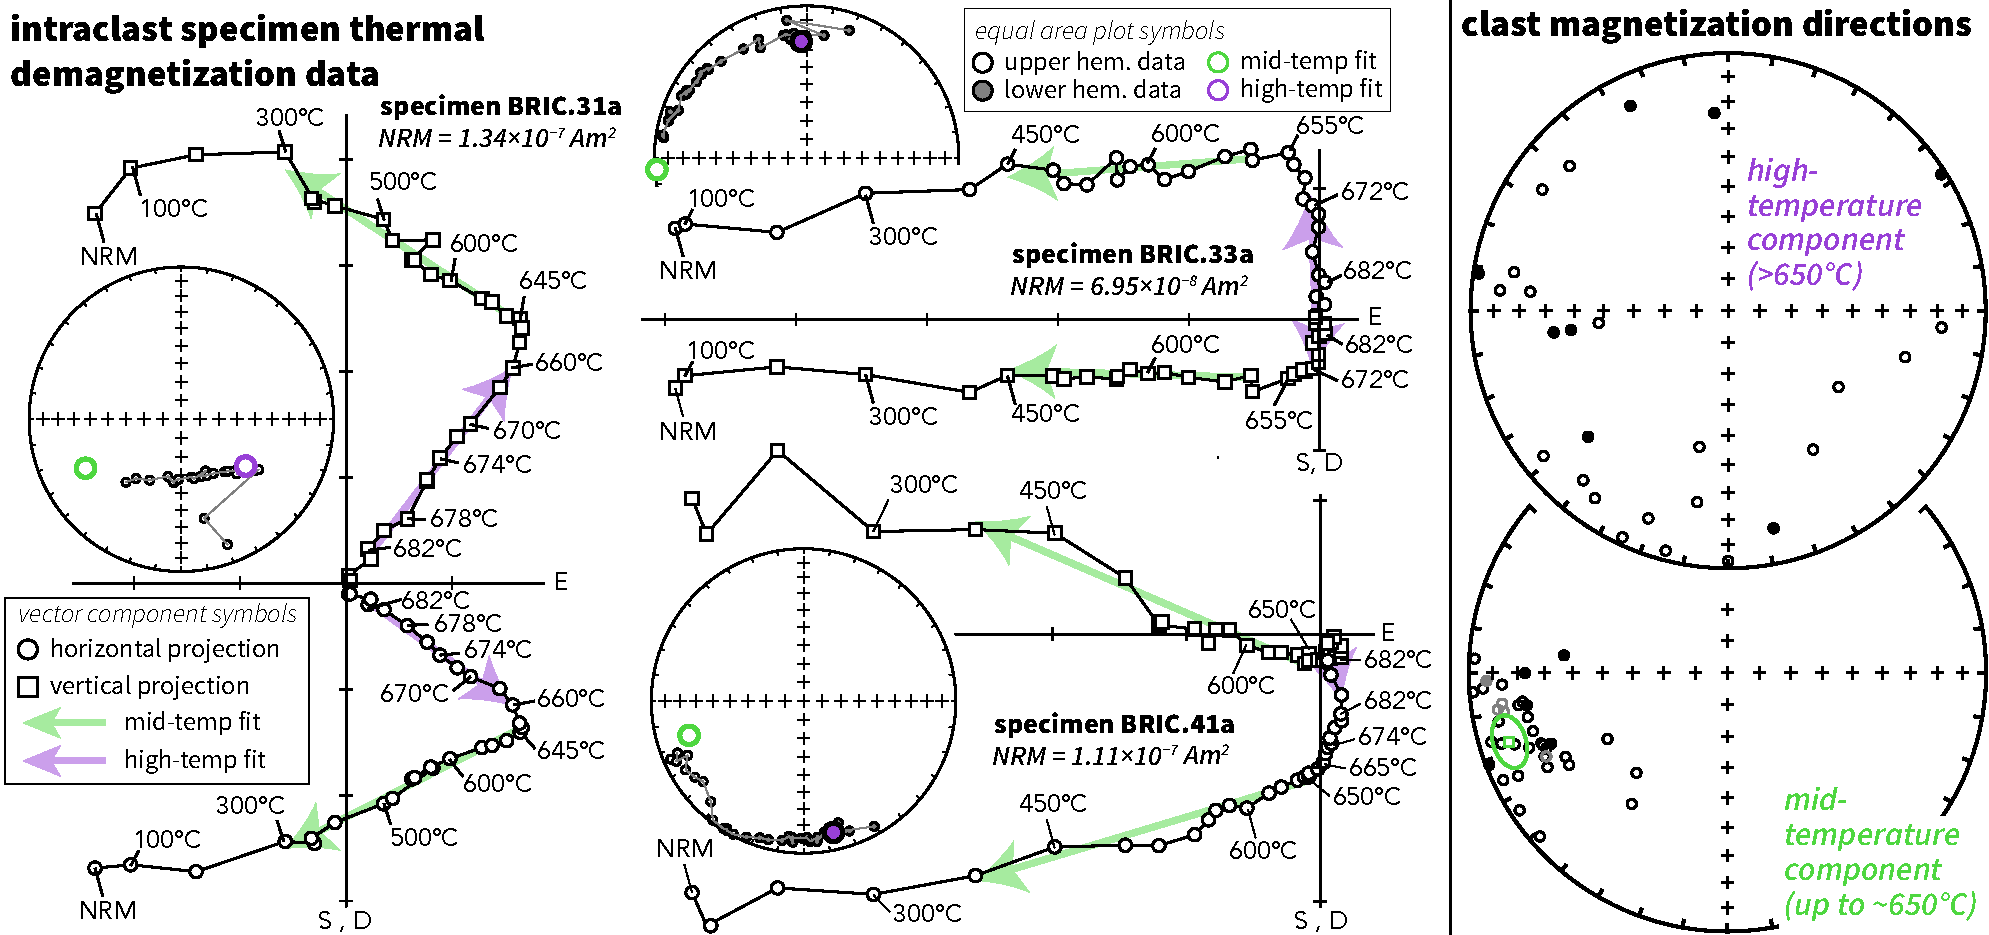
\includegraphics[width=\textwidth]{BRIC_pmag.pdf}
\caption{\small{Paleomagnetic data from intraclasts reveal a mid-temperature component that typically unblocks prior to 655\textdegree C and a high-temperature component that typically unblocks between 655\textdegree C and 687\textdegree C. These components are present as varying fractions of the overall remanence as seen in the three individual clasts for which data are shown on vector component plots and measurement-level equal area plots in tilt-corrected coordinates (developed using PmagPy; \citealp{Tauxe2016a}). The direction of the mid-temperature component is shown as purple arrows on the vector component plots and purple circles on the equal area plots while the high-temperature component is shown with green symbols. The mid-temperature component has a similar direction throughout the clasts as can be seen on the component directions equal area plots (mean declination: 252.4, inclination: -12.5, $\alpha_{95}$: 6.6). In contrast, the high-temperature component directions are dispersed.}}
\label{fig:intraclast_pmag}
\end{figure}

The clasts typically reveal two distinct magnetization directions. One direction was similar throughout the intraclasts and was typically removed between 200\textdegree C and 650\textdegree C (Fig. \ref{fig:intraclast_pmag}). This mid-temperature component is continuously unblocked between these temperatures with no or minimal downward inflection at $\sim$580\textdegree C that would indicate remanence associated with magnetite (Fig. \ref{fig:intraclast_pmag}). This component is directionally well-grouped indicating that it was acquired following deposition of the clasts (Fig. \ref{fig:intraclast_pmag}). The other component trends towards the origin and is removed by thermal demagnetization steps at the highest levels such that it typically can be fit by a least-square line between 665\textdegree C and 688\textdegree C. The relative magnitude of the components varies between intraclasts (Fig. \ref{fig:intraclast_pmag}). While the high-temperature component can sometimes be fit as a line with a lower temperature bound of 660\textdegree C (BRIC.31a in Fig. \ref{fig:intraclast_pmag}), due to overlapping unblocking temperatures between the mid-temperature and high-temperature components the lower bounds of the high-temperature fits sometimes need to be as high as 680\textdegree C (BRIC.41a in Fig. \ref{fig:intraclast_pmag}). Note that while the Ne\'el temperature of hematite is sometimes given as 675\textdegree C in the paleomagnetic literature, experimental data often shown the Ne\'el temperature to be as high as 690\textdegree C \citep{Ozdemir2006a}. There is typically a significant directional change in the specimen magnetization between the mid-temperature component and the high-temperature component (Fig. \ref{fig:intraclast_pmag}). As a result, 29 of the 39 analyzed intraclast specimens could be fit with distinct mid-temperature and high-temperature least-squares lines. An additional five specimens were undergoing directional change through the highest thermal demagnetization steps indicative of the presence of a distinct high-temperature component, but this component was not well-expressed enough to be fit. Five of the specimens showed no directional change and could be fit with a single mid-high-temperature component that is grouped with the mid-temperature component. In contrast to the well-grouped mid-temperature component, the high-temperature component directions are dispersed, indicating that the component was acquired prior to erosion and redeposition of the clasts. The high-temperature component directions are more dispersed in declination than inclination leading to a distribution that is not randomly dispersed on a sphere. Given that the clasts are tabular and were liberated along their depositional lamination and subsequently landed roughly bedding-parallel, it is to be expected that the rotations were largely around a vertical axis which would preferentially change declination.

Petrography on the intraclasts reveals two distinct populations of hematite (Fig. \ref{fig:intraclast_images}). One population is fine-grained pigmentary hematite present dominantly within the clay-sized matrix and rimming detrital silt-sized grains. The zones of pigmentary hematite within the matrix remain cloudy to high magnification indicating that the grains are submicron in size. The other population of hematite has similar sizes and shapes to other detrital silt-sized grains -- typically ranging from 2 to 50 $\mu$m in diameter. These hematite grains were identified through reflected light microscopy with their mineralogy supported by energy-dispersive x-ray spectroscopy and confirmed by electron backscatter diffraction. 

\section*{DISCUSSION}

Single-domain hematite grains have high coercivities ($>$150 mT; \citealp{Ozdemir2014a}) and high unblocking temperatures. As a result, populations of hematite within rocks are stable on long timescales, resistant to overprinting, and therefore attractive for paleomagnetic study. In contrast to magnetite, hematite grains retain stable single-domain behavior in crystals $>$1$\mu$m with the threshold to multidomain behavior occurring when grain diameters exceed $\sim$100$\mu$m \citep{Kletetschka2002a, Ozdemir2014a}. Hematite nanoparticles with diameters $<$30 nm have superparamagnetic behavior wherein thermal fluctuation energy overwhelms the ability of the grain to retain a stable magnetization at Earth surface temperatures \citep{Ozdemir2014a}. Hematite grains become progressively less influenced by thermal fluctuations as they reach grain sizes of a few hundred nanometers at which point they are stable up to temperatures approaching the N\'eel temperature of $\sim$685\textdegree C \citep{Swanson-Hysell2011a, Ozdemir2014a}. As a result, there is a strong relationship between grain volume and unblocking temperature that can be utilized to estimate grain size. A hematite population that is progressively unblocking at thermal demagnetization steps well below the N\'eel transition temperature, such as the mid-temperature component of the intraclasts, is comprised of grains within the $\sim$30 to $\sim$400 nm size range. This fine-grain size is consistent with the pigmentary phase observed within the intraclasts (Fig. \ref{fig:intraclast_images}).

Given the directional consistency of the mid-temperature component among the intraclasts, this component must have dominantly formed as a chemical remanent magnetization after the intraclasts were redeposited in the channel. Chemical remanent magnetization acquisition by pigmentary hematite would have occurred as hematite grains grew to sizes above the superparamagnetic to stable single-domain transition resulting in the wide range of unblocking temperatures that is observed. In contrast, given its sharp unblocking temperature close to the N\'eel temperature, the high-temperature component is dominantly held by hematite grains that are $>$400 nm such as the silt-sized hematite grains observed petrographically (Fig. \ref{fig:intraclast_images}). The high-temperature remanence component held by these grains was rotated along with the clasts indicating that it is primary and was acquired prior to the redeposition of the cohesive silt clasts. That this component is held by larger grains sizes supports it being a detrital remanent magnetization, rather than a chemical remanent magnetization that formed very early prior to clast erosion.

Oxidation of iron in aqueous environments often proceeds through the formation of fine-grained poorly crystalline ferrihydrite, which transforms to stable crystalline hematite at neutral pH on geologically short timescales \citep{Cudennec2006a}. The broad unblocking temperatures we observe for the chemical remanent magnetization in the Freda intraclasts are similar to those in hematite populations produced through experimental ferrihydrite to hematite conversion \citep{Jiang2015a}. The differential unblocking temperature spectra of the two components within the Freda intraclasts provides strong support for the argument of \cite{Jiang2015a} that chemical and detrital remanent magnetization can be distinguished; due to detrital remanence unblocking at the highest temperatures. However, it is also clear from the Freda intraclast data that while the detrital remanent magnetization can be well-isolated at temperatures as low as 650\textdegree C (specimen BRIC.31a in Fig. \ref{fig:intraclast_pmag}), the chemical remanent magnetization thermal unblocking spectra can overlap with that of the detrital remanence and extend up to temperatures closer to the N\'eel temperature (specimen BRIC.41a in Fig. \ref{fig:intraclast_pmag}). Therefore, to isolate primary remanence in red beds, best practice should be to proceed with very high resolution thermal demagnetization steps above 600\textdegree C, and particularly above 650\textdegree C. These intraclast data reveal that directional change at the highest unblocking temperatures provides an effective means to discriminate primary and secondary magnetizations within siltstones of the Freda formation and other red beds. The formation of coarse-grained secondary hematite can occur, particularly in high permeability lithologies and deeply weathered profiles. However, the isolation of primary detrital hematite in $>$1 billion-year-old siltstones lends confidence to magnetostratigraphic records and paleogeographic interpretations that are based on interpretations of primary magnetization in ancient red beds. 

\subsection*{ACKNOWLEDGEMENTS}
\footnotesize

This research was supported by the Esper S. Larsen, Jr. Research Fund and the National Science Foundation through grant EAR-1419894. SPS was supported by the Miller Institute for Basic Research in Science. The Wisconsin Department of Natural Resources granted a research and collection permit that enabled sampling within Copper Falls State Park. Oliver Abbitt assisted with field work, Taiyi Wang assisted with paleomagnetic analyses and Tim Teague provided technical support for EBSD analyses.

\singlespacing

\newpage

\bibliographystyle{gsabull}
\bibliography{../../references/allrefs}

\end{document}
